%-----------------------------------------------------------------------------
%
%               Template for sigplanconf LaTeX Class
%
% Name:         sigplanconf-template.tex
%
% Purpose:      A template for sigplanconf.cls, which is a LaTeX 2e class
%               file for SIGPLAN conference proceedings.
%
% Guide:        Refer to "Author's Guide to the ACM SIGPLAN Class,"
%               sigplanconf-guide.pdf
%
% Author:       Paul C. Anagnostopoulos
%               Windfall Software
%               978 371-2316
%               paul@windfall.com
%
% Created:      15 February 2005
%
%-----------------------------------------------------------------------------


\documentclass[10pt]{sigplanconf}

% The following \documentclass options may be useful:

% preprint      Remove this option only once the paper is in final form.
% 10pt          To set in 10-point type instead of 9-point.
% 11pt          To set in 11-point type instead of 9-point.
% authoryear    To obtain author/year citation style instead of numeric.

\usepackage{amsmath}
\usepackage{titlesec}

\begin{document}

\special{papersize=8.5in,11in}
\setlength{\pdfpageheight}{\paperheight}
\setlength{\pdfpagewidth}{\paperwidth}

%reduce a bit the spaces before or after section titles
\titlespacing*{\section}
{0pt}{0.8ex plus 1ex minus .2ex}{0.8ex plus .2ex}

\conferenceinfo{PaPoC'15}{April 21, 2015, Bordeaux, France} 
\copyrightyear{2015} 
\copyrightdata{978-1-4503-3238-5/15/04} 
\doi{http://dx.doi.org/10.1145/2745947.2745955}

% Uncomment one of the following two, if you are not going for the 
% traditional copyright transfer agreement.

%\exclusivelicense                % ACM gets exclusive license to publish, 
                                  % you retain copyright

%\permissiontopublish             % ACM gets nonexclusive license to publish
                                  % (paid open-access papers, 
                                  % short abstracts)

\titlebanner{banner above paper title}        % These are ignored unless
\preprintfooter{short description of paper}   % 'preprint' option specified.

\title{Minimizing Coordination in Replicated Systems\pagelimit{4}}

\authorinfo{Cheng~Li$^{\dagger}$ Jo{\~a}o~Leit{\~a}o$^{\ddagger}$ Allen~Clement$^{\dagger}$\thanks{currently working at Google} Nuno~Pregui{\c c}a$^{\ddagger}$ Rodrigo~Rodrigues$^{\ddagger}$}
	{$^{\dagger}$MPI-SWS $^{\ddagger}$NOVA LINCS / NOVA Univ.\ Lisbon\vspace{-1cm}}

%\authorinfo{Cheng Li}
%           {MPI-SWS}
%           {chengli@mpi-sws.org}
%\authorinfo{Jo{\~ a}o Leit{\~ a}o}
%           {NOVA-LINCS FCT UNL}
%           {jc.leitao@fct.unl.pt}
%\authorinfo{Allen Clement}
%           {Google Inc.}
%           {aclement@gmail.com}
%\authorinfo{Nuno Pregui{\c c}a}
%           {NOVA-LINCS FCT UNL}
%           {nuno.preguica@fct.unl.pt}
%\authorinfo{Rodrigo Rodrigues}
%           {NOVA-LINCS FCT UNL}
%           {rodrigo.rodrigues@fct.unl.pt}

\maketitle


\begin{abstract}
Replication has been widely adopted to build highly scalable services, but
the goal\changebars{}{ of achieving high performance} is often compromised by the
coordination required to ensure application-specific properties such as
state convergence and invariant preservation. In this paper, we propose a
principled mechanism to minimize coordination in replicated systems via the
following components: a) a notion of restriction over a pair of operations
that captures the fact that the two operations must be ordered w.r.t each
other in any partial order; b) a generic consistency model which, given a
set of restrictions, requires those restrictions to be met in all
admissible partial orders; c) principles for identifying a \changebars{minimal}{} set of
restrictions to ensure relevant properties\changebars{}{, where removing any restriction
from this set will no longer preserve all these properties}; and d) a
coordination service that dynamically \changebars{maps}{translates} restrictions to the most
efficient coordination protocols. \changebars{Our preliminary experience on analyzing
a few applications shows that we are able to infer a set of restrictions which 
comprises a minimal coordination plan.}{}
\end{abstract}

% \category{CR-number}{subcategory}{third-level}
% 
% % general terms are not compulsory anymore, 
% % you may leave them out
% \terms
% term1, term2
% 
% \keywords
% keyword1, keyword2

\section{Motivation and contributions}
\label{ch:redblue:sect:motiv}
As we mentioned in Chapter~\ref{chapter:intro}, scaling services over the Internet to meet the needs of an
ever-growing user base is challenging. In particular, in order to improve
user-perceived latency, which directly affects the quality of the user
experience, services replicate system state across geographically
diverse sites and direct users to the closest or least loaded site.


To avoid paying the performance penalty of synchronizing concurrent
actions across data centers, some systems, such as Amazon's
Dynamo~\cite{Decandia2007Dynamo}, resort to weaker consistency semantics
like eventual consistency where state can temporarily diverge.
Others, such as Yahoo!'s PNUTS~\cite{Cooper2008PNUTS}, avoid state
divergence due to the undesirable sets of behaviors it allows, by
requiring all \operations\ that update the service state to be
funneled through a primary site and thus incurring increased latency.

In order to address the inherent tension between improving performance and
maintaining meaningful consistency semantics, several approaches have been recently proposals 
for allowing multiple
  levels of consistency to
  coexist~\cite{Ladin1992LazyReplication,Sovran2011PSI,Singh2009Zeno}: some
  \operations\ can be executed optimistically, without synchronizing
  with concurrent actions at other sites, while others require a
  stronger consistency level and thus require cross-site
  synchronization. However, this places a high burden on the developer
  of the service, who must decide which \operations\ to assign which
  consistency levels. It is challenging to make such decisions since it requires reasoning about the consistency
  semantics of the overall system to ensure that the behaviors
  that are allowed by the different consistency levels satisfy the specification
  of the system.


In this chapter we present a comprehensive and principled approach to
this problem, aiming at enabling geo-replicated systems to be as fast
as possible, while ensuring that they are consistent when necessary. We make the following three contributions:
\begin{enumerate}
\item 
We propose a novel consistency definition called \RBc. The intuition
behind \RBc\ is that \blue\ operations execute locally and are lazily
replicated in an eventually consistent manner~\cite{Decandia2007Dynamo,Lloyd2011Causal,Terry1995Managing,
Mahajan2010Depot,Feldman2010Sporc,Shapiro2011Conflict,Singh2009Zeno}.\ \Red\ \operations, in contrast, are serialized with respect to each
other and require immediate cross-site coordination. In addition,
\RBc\ preserves
causality by ensuring that dependencies established when an
\operation\ is  invoked at its primary site are preserved as
the \operation\ is incorporated at other sites.

\item We identify the sufficient conditions under which \operations\ must be
  colored \red\ and may be colored \blue\ in order to ensure that
  application invariants are never violated and that all replicas
  converge on the same final state.  Intuitively, \operations\ that
  commute with all other \operations\ and do not impact invariants may
  be \blue; the remaining ones must be \red.

%an \operation\ may be \blue\ if it commutes with all other
%\operations\ and does not impact any invariants.

\item We observe that the commutativity requirement limits the space
  of potentially \blue\ \operations, provided that many \operations\ in real world applications
do not commute w.r.t each other. To address this limitation, we decompose \operations\ into two
  components: (1) a \initial\ \operation\ that identifies the changes
  the original \operation\ should make, but has no side effects
  itself, and (2) a \shadow\ \operation\ that performs the identified
  changes and is replicated to all sites. With this decomposition, only
  \shadow\ \operations\ are colored \red\ or \blue. This allows for a
  dynamic runtime classification of \operations\ and hence broadens the space
  of potentially \blue\ \operations.
\end{enumerate}

We built a system called \gemini\ that coordinates
\RedBlue\ replication, and use it to extend three applications to be
\RBct: the TPC-W and RUBiS benchmarks and the Quoddy social network.  Our evaluation using microbenchmarks and the three
applications shows that \RBc\ provides substantial latency and
throughput benefits.


%\begin{landscape}
\begin{table*}[t!]
\centering
\footnotesize
\begin{tabular}{c|c|c|c|c|c|c||c}
\hline
\specialcell{Consistency \\level} & Example systems & \specialcell{Immediate \\response} & \specialcell{State \\convergence} &  \specialcell{Single \\value} & \specialcell{General \\operations}  & \specialcell{Stable\\histories}& \specialcell{Classification \\strategy}\\
\hline
Strong & RSM~\cite{Lamport1978Time,Schneider1990RSM}                & no  & yes  & yes & yes & yes        & N/A\\
\hline
\specialcell{Timeline/\\snapshot} & \specialcell{PNUTS~\cite{Cooper2008PNUTS}, \\Megastore~\cite{Baker2011Megastore}}            & reads only  & yes & yes & yes & yes & N/A\\
\hline
Fork & SUNDR~\cite{Krohn2004Sundr}                                               & all ops & no  & yes  & yes & yes        & N/A\\
\hline
\multirow{3}{*}{Eventual}
& Bayou~\cite{Terry1995Managing}, Depot~\cite{Mahajan2010Depot} & all ops    & yes & no  & yes & yes         & N/A \\
                                   &  Sporc~\cite{Feldman2010Sporc}, CRDT~\cite{Shapiro2011Conflict}                 & all ops       & yes & yes & no & yes          & N/A \\
                                   & Zeno~\cite{Singh2009Zeno}, COPS~\cite{Lloyd2011Causal}  & weak/all ops      & yes & yes  & yes & no         & no / N/A\\
\hline
\multirow{2}{*}{\specialcell{Multi}}   
                                  
                                   & PSI~\cite{Sovran2011PSI}                        & cset         & yes & yes & partial & yes & no\\
                                   &lazy repl.~\cite{Ladin1992LazyReplication}, Horus~\cite{VanRenesse1996Horus}          & immediate/causal ops & yes & yes & yes & yes         & no\\
\hline
\RB\     & \gemini       & \Red\ ops & yes & yes & yes & yes & yes \\
\hline
\end{tabular}
\caption{Tradeoffs in geo-replicated systems and various consistency
  levels.}
\label{table:systemcompare}
\end{table*}
\end{landscape}

\section{Related work}%\pagelimit{1.5}}                                                    
\label{ch:redblue:sect:related}
\if 0
\paragraph{Target end-to-end properties.}
To frame the discussion of existing systems that may be used
for geo-rep\-li\-cat\-ion, we start by informally stating some
desirable properties that such solutions should support.\ The first property consists of ensuring a good user experience by
providing \textbf{low latency} access to the
service~\cite{Schurman2009latency}. Providing low latency access implies
that \operations\ should proceed after contacting a small number of
replicas, but this is at odds with other requirements that are often sacrificed by consistency
models that privilege low latency. The first such requirement is preserving
\textbf{caus\-al\-ity}, both in terms of the monotonicity of user requests
within a session and preserving causality across clients, which is key
to enabling natural semantics~\cite{Petersen1997Flexible}.  Second, it
is important for all \operations\
executed at one replica to be
propagated to all remaining replicas, a property we call
\textbf{eventual propagation}.\ Third, it is important that all
replicas that have executed the same set of \operations\ are in the
same state, i.e., that they exhibit \textbf{state convergence}; otherwise a quiescent system would return different views of the state
depending on which replicas the users connected to. Fourth, we also
want to avoid marked deviations from the conventional, single server
semantics. In particular, \operations\ should return a \textbf{single
  value}, precluding solutions that return a set of values
corresponding to the outcome of multiple concurrent updates; the
system should provide a set of \textbf{stable histories}, meaning that
user actions cannot be undone; and it should provide support for
\textbf{general \operations}, not restricting the type of
\transactions\ that can be executed.  Finally, the behavior of the
service must obey a service-dependent specification, which may be
defined as a set of \textbf{invariants} that must be preserved.
\fi

In this section, we compare several proposals of consistency definitions against our work
by analyzing which set of end-to-end properties described in Chapter~\ref{chapter:sysmodel} they offer.
Table~\ref{table:systemcompare} shows that different proposals strike different balances between
these target properties. While other consistency
definitions exist, we focus on the ones most closely related to the
problem of offering fast and consistent responses in geo-replicated
systems.

\paragraph{ Strong vs.\ weak consistency.}
On the strong consistency side of the spectrum there are definitions
like linearizability~\cite{Herlihy1990Linearizability}, where the
rep\-li\-cated system behaves like a single server that
serializes all \operations.\ This, however, requires coordination among rep\-li\-cas
to agree on the order in which \operations\ are executed, with the
corresponding overheads that are amplified in
geo-rep\-li\-ca\-tion scenarios. Somewhat more efficient are
timeline consistency in PNUTS~\cite{Cooper2008PNUTS} and
snapshot consistency in Megastore~\cite{Baker2011Megastore}. These
systems ensure that there is a
total order for updates to the service state, but give the option
of reading a
consistent but dated view of the service. %new
Similarly, Facebook has a primary site that handles updates
and a secondary site that acts as a read-only copy~\cite{Li2012Practical}.
This allows for fast reads executed at the closest site but writes still pay a penalty for serialization.  
%% These solutions provide fast reads but can result in degraded update
%% performance in situations, like social networking or online shopping
%% services, where a partitioning of the writers of each data item or
%% each group of data items is not easily achievable.
%% %% megastore and pnuts totally order writes but allow for stale reads
%%  The
%% Megastore~\cite{Baker11Megastore} system used by Google uses a
%% modified version of Paxos, requiring all replicas to be contacted
%% during write operations, but enables fast reads at a single replica;
%% % (and thus requires contacting a quorum
%% %of replicas) to serialize write \operations, but
%% %enables reads to read a consistent but dated view from a single replica.
%% \changebars{like PNUTS, this does not allow for fast writes.}{this has same benefits and drawbacks as PNUTS.}
%\rodrigo{Removable:} This system has the additional characteristic of grouping related
%data items in entity groups, and providing full ACID
%semantics within entity groups but lower consistency guarantees across
%the entity boundary. 
Fork consistency~\cite{Krohn2004Sundr, Mazieres2002Fork} addresses
the performance limitations of strong consistency by allowing users to
observe distinct causal histories.  The primary drawback of fork
consistency is that once replicas have forked, they can never be
reconciled.  Such approach is useful when building secure systems
but is not appropriate in the context of geo-replicating a single
service.

Eventual consistency~\cite{Terry1995Managing} is on the other end of the
spectrum. Eventual consistency is a catch-all phrase that covers any
system where replicas may diverge in the short term as long as the
divergence is eventually repaired and may or may not include
causality.  (See Saito and Shapiro~\cite{Saito2005Optimistic} for a
survey.)  In practice, as shown in Table~\ref{table:systemcompare},
systems that embrace weak consistency (e.g., eventual or causal consistency) have limitations. Some
systems waive the stable history property, either by rolling back
\operations\ and re-executing them in a different order at some of the
replicas~\cite{Singh2009Zeno}, or by resorting to a last writer wins
strategy, which often results in loss of one of the
  concurrent updates~\cite{Lloyd2011Causal}.  Other systems expose multiple values from
divergent branches in \operations\ replies either directly to the
client~\cite{Mahajan2010Depot,Decandia2007Dynamo} or to an
application-specific conflict resolution
procedure~\cite{Terry1995Managing}.  Finally, some systems restrict
\operations\ by assuming that all \operations\ in the system
commute~\cite{Feldman2010Sporc,Shapiro2011Conflict}, which might require
the programmer to rewrite or avoid using some \operations.

\paragraph{Coexistence of multiple consistency levels.} The solution we propose for addressing the tension between low latency
and strongly consistent responses is to allow different
\operations\ to run with different consistency
levels. Existing systems that used a similar approach include
Horus~\cite{VanRenesse1996Horus}, lazy replication~\cite{Ladin1992LazyReplication}, Zeno~\cite{Singh2009Zeno}, and
PSI~\cite{Sovran2011PSI}. However, none of these proposals guide the
service developer in choosing between the available consistency
levels.  In particular, developers must reason about wheth\-er their
choice leads to the desired service behavior, namely by ensuring that
invariants are preserved and that replica state does not diverge.
This can be challenging due to difficulties in identifying behaviors
allowed by a specific consistency level and understanding the
interplay between \operations\ running at different levels.  Our
research addresses this challenge, namely by defining a set of
conditions that precisely determine the appropriate
  consistency level for each operation.

\paragraph{Other related work.} Consistency rationing~\cite{Kraska2009ConsisRation} allows consistency
guarantees to be associated with data instead of \operations, and the
consistency level to be automatically switched at runtime between
weak consistency and serializability
based on specified policies.\ TACT~\cite{Yu2000TACT} consistency
bounds the amount of inconsistency of data items in an
application-specific manner, using the following metrics: numerical
error, order error and staleness. In contrast to these models, the
focus of our work is not on adapting the consistency levels of
particular data items at runtime, but instead on systematically
partitioning the space of \transactions\ according to their actions
and the desired system semantics.

One of the central aspects of our work is the notion of
\shadow\ \transactions, which increase \operation\ commutativity by
decoupling the decision of the side effects from their application to the state.
%This enables applications to make more use of fast \transactions. 
Some prior work also aims at increasing operation commutativity: Weihl exploited
com\-mut\-at\-iv\-ity-based concurrency control for abstract data types~\cite{Weihl1988Commutativity}; 
operational transformation~\cite{Ellis1989Concurrency,Feldman2010Sporc} extends
non-co\-mmutative \operations\ with a
transformation that makes them commute; Conflict-free Replicated Data
Types (CRDTs)~\cite{Shapiro2011Conflict} design \operations\ that
commute by construction; Gray~\cite{Gray1981NestedTransactions} proposed
an open nested transaction model that uses commutative compensating
transactions to revert the effects of aborted transactions without
rolling back the transactions that have seen their results and already
committed; delta transactions~\cite{deltaTxBlog} divide a transaction
into smaller pieces that commute with each other to reduce the
serializability requirements.  Our proposal of
\shadow\ \transactions\ can be seen as an extension to these concepts,
providing a different way of broadening the scope of potentially commutative
\transactions. There exist other proposals that also decouple the
execution into two parts, namely two-tier
replication~\cite{Gray1996Dangers} and CRDT
downstreams~\cite{Shapiro2011Conflict}. In contrast to these proposals, for
  each \operation, we may generate different
  \shadow\ \operations\ based on the specifics of the execution,
which can run under different consistency levels. As a result, the decomposition enables a
dynamic runtime classification of consistency levels, and
allows applications to make more use of fast \operations.


%\section{System models}
\changebars{We assume a distributed system with state fully replicated across
$k$ sites denoted $\textit{site}_0\ldots \textit{site}_{k-1}$. Each site
hosts a replica, and each replica behaves a deterministic state machine model. Any
service running on the top of that replicated system defines a set of
desirable target properties, in order to deliver a meaningful and good user experience. 
The most representative and important properties are three pillars: a) {\bf Causality}---the
service ensures the monotonicity of user requests within a session and preserving causal dependencies
across clients; b) {\bf State convergence}---all replicas that have executed the same set of operations are
in the same state; c) {\bf Invariant preservation}---the behavior of the system
must obey its specification, which may be defined as a set of invariants that must
be preserved, e.g., that no two users receive the same user id when registering.}{}

\section{Partial Order-Restriction Consistency}
\label{ch:por:sect:pordef}
In this section we introduce \PRCNF\ (or short, \PRCN), a novel consistency model that allows
the developer to reason about various consistency requirements in a single
system. The key intuition behind our proposal is that this model is generic and 
can be perceived as a set of restrictions imposed over admissible partial orders 
across the operations of a replicated system.

\subsection{Defining \PRCN}
We formulate \PRCN\ by following the same methodology we used for \RBCN\ (Seen in Chapter~\ref{chapter:redblue}).
The definition of \PRCN\ includes three important components: (1) a set of restrictions, which
specifies the visibility relations between pair-wise operations; (2) a Restricted Partial order (or short, R-Order), which
establishes a (global) partial order of operations respecting operation visibility relations; and (3) a set of site-specific causal serializations,
which corresponds to total orders in which the operations are locally applied. We define
these components formally as follows:

\begin{mydef}
\textbf{Restriction: } Given a set of operations $U$, a restriction is a symmetric binary relation on $U\times U$
\footnote{This definition is analogous to the conflict relation in Generic Broadcast~\cite{Pedone99genericbroadcast}.}.
\label{def:restr}
\end{mydef}

For any two operations $u$ and $v$ in $U$, if there exists a restriction relation $r(u, v)$, 
then they must be ordered in any partial order $\prec$, i.e., $u\prec v \vee v\prec u$. We capture this point
in the following definition.

\begin{mydef}
\textbf{Restricted Partial Order (or short, R-Order): } Given a
set of operations $U$, and a set of restrictions $R$ over $U$, an R-Order is a partial order
$O = (U, \prec)$ with the following constraint: $\forall u, v\in U,$ $r(u, v)\in R$ $\implies u\prec v\vee v\prec u$.
\label{def:rorder}
\end{mydef}

We also say that restrictions in $R$ are met in the corresponding R-Order if this order
satisfies the above definition. Similar to \RBCN, every site (replica) executes operations following a linear
extension of the global R-Order. The following definition defines what linear extensions are allowed with respect to
a given R-Order.

\begin{mydef}
\textbf{Legal serialization: } $O' = (U, <)$ is a legal serialization of R-Order $O = (U, \prec)$
if $O'$ is a linear extension of $O$; i.e., $<$ is a total order compatible with the partial order defined by $\prec$.
\label{def:legalserial}
\end{mydef}

As introduced in Chapter~\ref{chapter:redblue}, our proposal of splitting operations into pairs of generator and shadow
operations changes the traditional state machine replication definitions. In this work, we also embrace
the shadow operation concept so that we can reduce the number of required restrictions for ensuring
state convergence. With this change,
when user requests are accepted by any site, that site executes their generator operations and 
creates corresponding shadow operations. In addition, every site also 
incorporates remote shadow operations that are shipped from all other sites into its local serialization. 
We denote $U$ a set of shadow operations. For a site $i$,
its generator operation set is denoted by $V_{i}$. The following definition captures the application
of both local and remote shadow operations at a site $i$.


\begin{mydef}
\textbf{Causal legal serialization: } Given a site $i$, a R-Order $O=(U, \prec)$ and the set of generator operations $V_i$ received at site $i$, we say that $O_i = (U\cup V_{i}, <_i)$ is an i-causal legal serialization (or short, a
causal serialization) of $O$ if
\begin{itemize}
\item $O_i$ is a total order;
\item $(U,<_i)$ is a legal serialization of $O$;
\item For any $h_v(S)\in U$ generated by $g_v\in V_i$, $S$ is the
  state obtained after applying the sequence of
  shadow operations preceding $g_v$ in $O_i$;
\item For any $g_v\in V_i$ and $h_u(S) \in U$, $h_u(S)<_{i}g_v$ in $O_i$
  iff $h_u(S) \prec h_v(S')$ in $O$.
\end{itemize}
\label{def:causalserial}
\end{mydef}

%Since generator operations have no side effects, in order to make proofs easy to follow, we simplify $O_i = (U\cup V_{i}, <_i)$ to $O'_i = (U, <_i)$ by removing generator operations in $V_{i}$ from $O_i$. If $O_i = (U\cup V_{i}, <_i)$ is an $i$-causal serialization of a R-Order $O$, then
%the simplified version $O'_i = (U, <_i)$ is too.

A replicated system with $k$ sites is then \PRCAJ\ if every site applies a
causal serialization of the same global R-Order $O$.

\begin{mydef}
\textbf{\PRCNF\ (or short, \PRCN):} A replicated system $\mathscr{S}$ with a set of restrictions $R$ is \PRCAJ\ if 
each site $i$ applies shadow operations according to an $i$-causal serialization of R-Order $O$.
\label{def:porconsistency}
\end{mydef}


\subsection{Expressiveness} The intuition behind the \PRCN\ model is that the model can be viewed as a
parametrized function, which takes restrictions as input, and outputs
a particular consistency model where the restrictions must be met in any partial order.
To demonstrate the power of \PRCN,
we use it to express many different consistency requirements. 
For causal consistency~\cite{Lloyd2011Causal} (excluding any restrictions to provide session guarantees), 
the restriction set is empty, since causality is already preserved in the definition 
of \PRCN\ by having $u \prec v \wedge v \prec w \implies u < w$. 
Regarding \RBCN, to capture the notion of strongly consistent (red) operations, we define 
the following restriction set: for any pair of operations $u$, $v$, if $u$ and $v$ are strongly consistent, 
we have $r(u,v)$. Serializability~\cite{Bernstein1987CCR} totally orders all
operations, so its restriction set is as follows: for any pair of operations $u$, $v$, we have $r(u, v)$.

\section{Restriction inference}
\label{ch:por:sect:infer}
When replicating a service under \PRCN, the first step is to
infer restrictions to ensure two important system 
properties, namely, state convergence and invariant preservation. 
The major challenge we face is to identify a small set of restrictions for
making the replicated service eventually converge and never violate invariants so
that the amount of required coordination is minimal.
With regard to state convergence, we take a similar
methodology adopted in prior research~\cite{Shapiro2011CRDTs,
Li2012RedBlue, Li2014SIEVE}, which is to check operation commutativity.
However, unlike \RBCN, under which all operations that are not globally commutative must be totally ordered,
\PRCN\ only requires that an operation must be ordered w.r.t another one if
they do not commute.

To always preserve application-specific invariants,
instead of totally ordering all non-invariant safe
shadow operations, i.e., those that potentially transition from a valid state
to an invalid one, we try to isolate
the operations that exclusively contribute to an invariant violation from
the rest. To do so, we introduce
a new concept, called an {\tt I-conflict set}, which defines a minimal set of
shadow operations that lead to an invariant violation when they are running
concurrently in a coordination-free manner. By minimal, we mean that by removing 
any shadow operation from such a set, the violation will no longer persist. 
To identify a minimal set of restrictions, we first perform an analysis over any subsets of the shadow 
operation set to discover all {\tt I-conflict} sets. Then, for any such set, adding a 
restriction between any pair of its operations is sufficient to eliminate 
the problematic executions.

Next, we present the definitions, theorems, proofs and algorithms
regarding the restriction set identification and refinement.

\subsection{State convergence}
\label{sec:properties:converge}
A PoR-consistent replicated system is state convergent if all its replicas reach
the same final state when the system becomes quiescent, i.e., for any pair of causal legal serializations
of any R-Order, $L_{1}$ and $L_{2}$, we have $S_0(L_1) = S_0(L_2)$, where $S_0$ is the valid initial state. We
state the necessary and sufficient conditions to achieve this in the following theorem.

%\begin{mydef}
%\textbf{Convergence}: A system $\mathscr{S}$ starting from an initial state $S$ and with a set of restrictions $R$ is convergent if,
%for any execution of $\mathscr{S}$ and its corresponding R-Order $O$, any two legal serializations of $O$, $L_{1}$ and $L_{2}$, are state convergent, i.e., $S(L_{1}) = S(L_{2})$.
%\label{def:converge}
%\end{mydef}

%\cheng{Why we use the term legal serialization instead of causal legal serialization is because that the number of replicas can be dynamically changed.}

\begin{theorem}
\label{theorem:convergence}
\emph{(Convergence Theorem)}
A \PRCAJ\ system $\mathscr{S}$ with a set of restrictions $R$ is \textbf{convergent}, if and only if,
for any pair of its shadow operations $u$ and $v$, $r(u, v) \in R$ if $u$ and $v$ don't commute.
\end{theorem}

In order to prove this theorem, we need the assistance from three lemmas introduced in Chapter~\ref{chapter:redblue}, namely,
Lemmas~\ref{lem:canSwap}, ~\ref{lem:adjexists} and ~\ref{lem:adjacentconvergent}. The first lemma asserts that,                             
given a legal serialization, swapping two adjacent
shadow operations in this serialization that are not ordered by the R-Order
results in another legal serialization. The second lemma asserts that given an R-Order and one of its legal serializations, if there exists
a pair of shadow operations $u$ and $v$ that are not ordered by the R-Order, then there exists an adjacent
pair of shadow operations between $u$ and $v$ in that serialization that are not ordered
by the R-Order. The third lemma asserts that two legal serializations that differ
in the order of exactly one pair of adjacent shadow operations are state
convergent, if all blue operations are globally commutative. The first two lemmas remain valid under \PRCN\ since their proofs
remain unchanged. However, we have to change the third lemma since \RBCN\ archieves state convergence by requiring
all blue shadow operations to commute but \PRCN\ only needs any pair of unordered shadow operations
to commute. We apply the following changes to Lemma~\ref{lem:adjacentconvergent},
which results in a new lemma (Lemma~\ref{lem:poradjacentconvergent}).
\if 0
%\begin{lemma}\label{lem:canSwap}
% Given a legal serialization $O_i=(U,<_i)$ of R-Order $O=(U,\prec)$
% with shadow operations $u,v\in U$ such that $u<_iv$ and $u \not\prec v$ and
% there exists no $s$ such that $u<_{i}s<_{i}v$, and let $P=\{ p | p \in U \wedge p <_i u\}$
% and $Q=\{q | q \in U \wedge v <_i q\}$. The serialization $O_k=(U,<_k)$ where
%   \begin{itemize}
%     \item $\forall p,q\in P \cup Q: p<_kq
%       \Longleftrightarrow p<_iq$,
%   \item $\forall p \in P: p <_k v$,
%   \item $v<_k u$,
%   \item $\forall q \in Q: u <_k q$
%  \end{itemize}
%  is a legal serialization of $O$.
%  \end{lemma}
% \begin{lemma}\label{lem:adjexists}
% Given a legal serialization $O_i=(U,<_i)$ of R-Order $O=(U,\prec)$, if
% $\exists u,v\in U$ such that $u<_i v$ and $u\not\prec v$,
% let $U' = \{u,v\} \cup \{q|u<_i q\wedge q<_i v\}$, then $\exists r, s \in U'$ such that $r<_i s \wedge$ $r\not\prec s$ $\wedge \not\exists p \in U': r<_i p\wedge p <_i s$.
% \end{lemma}
\fi

\begin{lemma}\label{lem:poradjacentconvergent}
Assume $O_i=(U,<_i)$ and $O_j=(U,<_j)$ are both legal
serializations of R-Order $O=(U,\prec)$ that are identical except for
two adjacent operations $u$ and $v$ such that $u<_iv$ and $v<_ju$ and that $u$ and $v$ commute. Then
$S(O_i)=S(O_j)$.
\end{lemma}

The above lemma asserts that two legal serializations that differ
in the order of exactly one pair of adjacent shadow operations are state 
convergent, if the two operations commute. We introduce the proof 
of Lemma~\ref{lem:poradjacentconvergent} as follows.

\noindent{\bf Proof:} Let $P$ and $Q$ be the greatest common prefix and suffix
of $O_i$ and $O_j$, respectively.  Further, let $S_P=S_0(P)$,
$S_{uv}=S_P+u+v$, and $S_{vu}=S_P+v+u$. By the definition of operation commutativity,
$S_{uv} = S_{vu}$. It then follows the definition
of deterministic state machine that $S_{uv}(Q) = S_{vu}(Q)$. 
By the definition of legal serialization (Definition~\ref{def:legalserial}),
the final state reached by sequentially executing operations in $O_{i}$ 
against $S_0$ according to $<$ is equal to the final state obtained by 
sequentially applying operations in $Q$ against $S_{uv}$ according to $<$, namely $S_0(O_i)=S_{uv}(Q)$. By a
similar argument, we know $S_0(O_j)=S_{vu}(Q)$. Finally, we have $S_0(O_i)=S_0(O_j)$.
\qed

After adapting these lemmas from Chapter~\ref{chapter:redblue} to \PRCN, we use
them to construct the proof of the state convergence theorem (Theorem~\ref{theorem:convergence}) as follows:

\noindent{\bf Proof:}
($\Leftarrow$:) We first show that if for any pair of non-commuting operations of $\mathscr{S}$,
a restriction between this pair of operations is in $R$, then the \PRCAJ\ system $\mathscr{S}$ is convergent. 
To prove this, it is sufficient to show that any pair of legal serializations of their underlying R-Order $O$ 
is state convergent. Let $O_{i}$ and $O_{j}$ be two legal serializations of $O$. Let $S$ be the initial state.
There are two cases to consider:

{\bf Case 1:} $O_i = O_j$.  The underlying deterministic state
machine ensures that $S(O_i)=S(O_j)$.

{\bf Case 2:} $O_i \neq O_j$, in which case $\exists u,v\in U$
such that $u<_i v$ and $v<_j u$. Since both $O_i$ and $O_j$ are
legal serializations of $O$, it follows that $u\not\prec v$ and
$v\not\prec u$. It then follows from Lemma~\ref{lem:adjexists} that we
can find an adjacent pair of operations $r, s$ in both $O_i$ and $O_j$ such
that $r<_i s \wedge s<_j r \wedge r\not\prec s \wedge s\not\prec r$. 
We construct a new serialization $O_{i+1}$ by duplicating $O_i$ but swapping the 
order of $r$ and $s$ in $O_{i+1}$, i.e., $r<_i s \wedge s<_{i+1} r$. By Lemma~\ref{lem:canSwap}, 
$O_{i+1}$ is also a legal serialization of $O$. It then follows from the hypothesis that $r$ and $s$
commute and from Lemma~\ref{lem:adjacentconvergent} that $O_i$ and $O_{i+1}$ are convergent.

If $O_{i+1} \neq O_j$, we continue the construction by finding
an adjacent pair of operations whose order is different in $O_{i+1}$, $O_j$. By swapping
the two operations, we obtain another legal serialization $O_{i+2}$. We can then continue to swap
all such adjacent pairs until the last constructed serialization
is equal to $O_j$. This is achievable since at every step the number of operation pairs in the corresponding newly constructed legal serialization 
whose orders are different in $O_j$ decreases.
At the end, the construction process results in a chain of legal
serializations where the first one is $O_i$ and the last is $O_j$, and any consecutive pair of legal serializations
is identical except for the order of an adjacent pair of elements. It then follows
Lemma~\ref{lem:adjacentconvergent} that every consecutive pair of
serializations in the chain is state convergent, thus $S_0(O_i) = S_0(O_j)$.


\noindent ($\Rightarrow$:) (Proof by Contradiction.) We show that if a \PRCAJ\ system $\mathscr{S}$ 
with a restriction set $R$ is convergent, then for any pair of non-commuting shadow operations, there must exist
a restriction confining the two operations in $R$. Since $\mathscr{S}$ is convergent, we know that for any R-Order of $\mathscr{S}$, any pair of legal serializations of that R-Order are convergent. We assume by contradiction that there exist two
shadow operations $u, v$ such that they don't commute and $r(u, v) \not\in R$. By the definition of commutativity, there exists
a state $S$ such that $S+u+v \neq S+v+u$. We can find a state $S_0$ and a legal serialization of $\mathscr{S}$, $O_1(P, <)$, such that $S_0(P) = S$. Then,
we can construct a R-Order $O(U, \prec)$, where 

\begin{itemize}
\item $U = P\cup\{u, v\}$;
\item for any pair of operations in $P$, $m$ and $n$, $m<n \Longleftrightarrow m\prec n$;
\item for any operation $m$ in $P$, $m \prec u$ and $m \prec v$.
\end{itemize}  

$u, v$ are the maximal elements of $O$. It follows from the definition of causal legal serialization (Definition~\ref{def:causalserial}) that
we can construct two legal serializations $L_1$ and $L_2$ of $O$ such that $L_1 = P + u + v$ and $L_2 = P + v + u$. 
As $S_0(L_1) = S_0(P + u +v)$, $S_0(L_1) = S_0(P) + u +v$. It follows from $S_0(P) = S$ that $S_0(L_1) = S+u+v$. By a similar argument, $S_0(L_2) = S+v+u$.
It then follows from $S+u+v \neq S+v+u$ that $S_0(L_1)\neq S_0(L_2)$. As $L_1$ and $L_2$ are not convergent, $\mathscr{S}$ is not convergent. Contradiction is
found.
\qed


\subsection{Invariant preservation}
\label{sec:properties:inv}
As presented in the RedBlue consistency chapter (Chapter~\ref{chapter:redblue}), the methodology
for identifying restrictions imposed on RedBlue orders for maintaining invariants is to check if
a shadow operation is invariant safe or not. If not, to avoid invariant 
violations, the generation and replication of all non-invariant safe shadow operations must be coordinated. 
However, we observed that for some non-invariant safe shadow operations $u$, the corresponding violation
only happens when a particular subset of non-invariant safe shadow operations are not partially ordered. 
To eliminate all invariant violating executions with a minimal amount of coordination, therefore, 
we need to precisely define, for each violation, the minimal
set of non-invariant safe shadow operations that are involved. We call this
set an {\tt invariant-conflict operation set}, or short, {\tt I-conflict set}. We formally define this 
as follows.

\if 0
\begin{mydef}
[Invariant safe condition] Given a shadow operation $h_{u}(S)$, its invariant safe
condition is a function $isc(S')$ of all valid state $S'$ and $S$ such that $isc(S')$ holds iff
$S' + h_{u}(S)$ is also a valid state. 
\label{def:isafecond}
\end{mydef}

For simplicity, for any shadow operation $u$, we denote $u.isc$ as its invariant preserving condition. Apparently,
if $u$ is an invariant safe shadow operation, then $u.isc = $ {\tt true} w.r.t all valid state.
\fi
\changebars{
\begin{mydef}
[Invariant-conflict operation set] A set of
shadow operations $G$ is an invariant-conflict operation set (or short, I-conflict set), if
the following conditions are met:
\begin{itemize}
 \item $\forall u \in G$, $u$ is non-invariant safe;
 \item $|G| > 1$;
 \item $\forall u \in G$, $\forall$ sequence P consisting of all shadow operations in G except u, i.e.,
$P = (G \setminus \{u\}, <)$, and $\exists$ a reachable and valid state $S$, s.t. $S(P)$ is valid, and
$S(P + u)$ is invalid.
\end{itemize}
\label{def:iconflictset}
\end{mydef}
}{}

In the above definition, the last point asserts that
$G$ is minimal, i.e., removing one shadow operation from it will no
longer lead to invariant violations. We will use the following example to illustrate
the importance of minimality. Imagine that we have an auction on an item $i$ 
being replicated across three sites such as US, UK and DE,
and having initially a $5$ dollar bid from $Charlie$. Suppose also that three shadow operations,
namely, $placeBid'(i, Bob, 10)$, $placeBid'(i, Alice, 15)$, and 
$closeAuction'(i)$ are accepted concurrently at the three locations, respectively. 
After applying all of them against the same initial state at every site,
we end up with an invalid state, where $Charlie$ rather than $Bob$ and $Alice$ won
the auction. This invariant violating execution
involves three concurrent shadow operations, but one of the two bid placing shadow
operations is not necessarily to be included in $G$, as even after excluding
the request from either $Bob$ or $Alice$, the violation still remains. \changebars{According
to Definition~\ref{def:iconflictset}, $\{ placeBid', closeAuction'\}$ is an \texttt{I-conflict set},
while $\{placeBid', placeBid', closeAuction'\}$ is not. Intuitively, avoiding invariant
violations is to prevent all operations from the corresponding \texttt{I-conflict} set
from running in a coordination-free manner. The minimality property enforced in the \texttt{I-conflict set}
definition allows us to avoid adding unnecessary restrictions.}{}  

Based on the above definition, we then can
 formulate the invariant preservation property into the following theorem.

\if 0
\begin{figure*}[t!]
\begin{minipage}[t]{0.5\textwidth}
\subfloat[R-Order $O$ of an execution $E$, which violates invariants]{\label{fig:invarexamplerorder}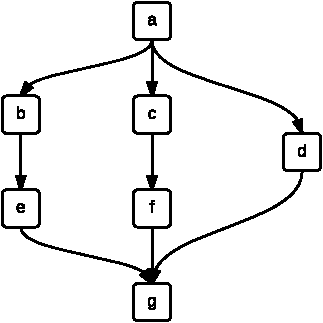
\includegraphics[width=0.8\textwidth]{./por/figures/por_invariant_preserving_chart_rorder.pdf}}
\end{minipage}
\begin{minipage}[t]{0.5\textwidth}
\centering
\subfloat[Shortest linear prefix of $O$ observing invalid state]{\label{fig:invarexamplerprefix}
\includegraphics[width=1.0\textwidth]{./por/figures/por_invariant_preserving_chart_P.pdf}}\\
\subfloat[R-Order $O'$ of $P$]{\label{fig:invarexampleshortestrorder}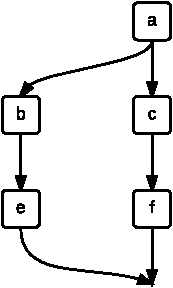
\includegraphics[width=0.3\textwidth]{./por/figures/por_invariant_preserving_chart_shortest_rorder.pdf}}\\
\subfloat[A permutation of $P$, where $T = f+e$ is the suffix]{\label{fig:invarexamplerpermu}
\includegraphics[width=1.0\textwidth]{./por/figures/por_invariant_preserving_chart_permu.pdf}}
\end{minipage}
\caption{Illustrative example for the proof of the invariant preservation theorem~\ref{theorem:invpreserve}. Rectangle boxes represent
shadow operations. The set $\{e, f\}$ is I-conflict set, while $\{b, c\}$ is not. $d$ is invariant safe.}
\label{fig:invarexample}
\end{figure*}
\fi

\begin{theorem}
{\bf Invariant preservation theorem:} Given a \PRCAJ\ system $\mathscr{S}$
with a set of restrictions
$R_{\mathscr{S}}$, for any execution of $\mathscr{S}$ that starts from a valid state, no site
is ever in an invalid state, if the following conditions are met:
\begin{itemize}
 \item for any its {\tt I-conflict} set $G$, there exists
a restriction $r(u, v)$ in $R_{\mathscr{S}}$, for at least one pair of shadow operations $u, v \in G$; and
 \item for any pair of shadow operations $u$ and $v$, $r(u, v)$ in  $R_{\mathscr{S}}$ if $u$ and $v$ don't commute.
\end{itemize}

\label{theorem:invpreserve}
\end{theorem}
\if 0
To prove the above theorem, we need to introduce the following lemma, which states that
in a legal serialization, for any shadow operation $h_u(S)$, let $S'$ be the state before
executing $h_u(S)$, if $S \neq S'$, then there must exist at least a shadow operation $v$ such that
$u$ and $v$ are not ordered w.r.t the corresponding R-Order, i.e., $u$ and $v$ are running concurrently.

\begin{lemma}\label{lem:concurrentexists}
Let $O_i=(U,<_i)$ be  a legal serialization of R-Order $O=(U,\prec)$, 
where $\forall m, n\in U, m\not\prec n \wedge n\not\prec m \implies $ $m$ and $n$
commute. Let $S_0$ be the initial state, for any
shadow operation $h_u(S) \in U$, let $S'$ be the state obtained by sequentially applying all shadow
operations in $U$ that precede $h_u(S)$ according to $<_i$ against $S_0$.
If $S \neq S'$, then $\exists v\in U$ such that $h_u(S)\not\prec v$ and $v\not\prec h_u(S)$.
\end{lemma}

\noindent{\bf Proof:}
We assume by contradiction that $S \neq S'$ but $\not\exists v\in U$ such that $h_u(S)\not\prec v$ and $v\not\prec h_u(S)$. This implies
that $\forall v \in U$, if $v \neq h_u(S)$, then $v \prec h_u(S)$ or $h_u(S) \prec v$. It then follows from \PRCN\ (Def~\ref{def:porconsistency})
and the legal serialization definition (Def~\ref{def:legalserial}) that for any legal serialization $L$ of $O$, $h_u(S)$ partitions
$L$ into two sequences $P$ and $Q$, where $P$ is a sequence containing exactly all shadow operations preceding $h_u(S)$ according to $\prec$ 
and $Q$ is a sequence containing exactly all shadow operations following $v$ according to $\prec$. 
Let $L_{c}$ the causal serialization of $O$ from site $i$, which is the primary site of the generator operation $g_u$ of $h_u(S)$. 
Let $L_c = P_c + h_u(S) + Q_c$. It follows from the definition of causal legal serialization (Def ~\ref{def:causalserial}) that $S_0(P_c) = S$.
Let $L_1$ and $L_2$ be two legal serializations of $O$ such that $L_1 = P_1 + h_u(S) + Q_1$ and $L_2 = P_2 + h_u(S) + Q_2$. 
It then follows from Lemma~\ref{lem:canSwap}, ~\ref{lem:adjexists}, ~\ref{lem:adjacentconvergent}
and the assertion that any pair of concurrent shadow operations in $O$ commute that $S_0(P_1) = S_0(P_2) = S_0(P_c)$. 
As a result, in every legal serialization including $L_c$, $S' = S$. Contradiction is found.
 \qed
\fi

%With the above lemma, we can prove the invariant preservation theorem as follows:
We prove the invariant preserving theorem by contradiction as follows:
\changebars{
\noindent{\bf Proof:} 
We assume by contradiction that
invariant violations are possible with a sufficient set of restrictions
$R_{\mathscr{S}}$ in place. Let $E$ be an invariant violating execution of $\mathscr{S}$ 
and let $O(U, \prec)$ be the R-Order of $E$. Let $O'(U_P, \prec)$
be a smallest R-Order that triggers the violation. $U_P \subset U$. Let $P(U_P,<)$ be a legal
serialization of R-Order $O'$. As $P$ violates the corresponding invariant, $S_{0}(P)$ is invalid. If $U_P$ is empty,
then $S_{0}(P) = S_0$, and $P$ is in a valid state. This violates the assumption
that $P$ is in an invalid state. The theorem is proved.

Then we consider that $U_P$ is non-empty. Let $G$ be the set of shadow operations
that are maximal according to $O'(U_P, \prec)$, i.e., $G \subset U_P$,
and $u \in G \Leftrightarrow \not\exists v \in U_P $ s.t. $u \prec v$.
The fact $U_P$ is not empty implies that $G$ is not empty as well. 

We first consider the case that $G$ contains invariant-safe shadow operations. Let $v$
be such an invariant safe shadow operation in $G$. If $v$ is not the last operation in $P$,
then it follows from Lemma~\ref{lem:canSwap}, ~\ref{lem:adjexists} and
the assertion that any pair of shadow operations that are not ordered in $\prec$ commute
w.r.t each other that we can swap $v$ and any shadow operation $u$, s.t. $u \in G$, $u \neq v$ and $v < u$.
This swapping process allows us to produce a new legal serialization $Q$ of the R-Order $O'$, where
$v$ appears as the last operation, i.e., $Q = Q' + v$. It also follows
from Lemma~\ref{lem:poradjacentconvergent} that $S_0(Q) = S_0(P)$. As $S_0(P)$ is invalid and $S_0(Q') + v = S_0(Q)$, 
$S_0(Q') + v$ is invalid. It then follows from the fact $v$ is invariant safe and the
invariant safe shadow operation definition (Def~\ref{def:isafeop}) that the state before applying $v$ must be invalid,
i.e., $S_0(Q')$ is not valid. This implies that there exists a smaller R-Order
$O''(U_P\setminus\{v\}, \prec)$ than $O'(U_P, \prec)$ that triggers the corresponding invariant. 
It contradicts with our assumption that $O'$ is a smallest R-Order observing invalid state.
Therefore, we only need to analyze the case when all shadow operations in $G$ are non-invariant safe.

We continue by checking if $|G| = 1$, i.e., $G$ contains a single non-invariant safe shadow operation. Let $v$ be that operation.
Let $L$ be the causal legal serialization of $O'$ from site $i$, where the generator of $v$ was executed.
Since $v$ is the only maximal element in $O'$, $L = L' + v$. It also follows from Lemma~\ref{lem:canSwap}, ~\ref{lem:adjexists},
Lemma~\ref{lem:poradjacentconvergent} and the assertion that any pair of unordered shadow operations commute that
$S_0(P) = S_0(L' + v)$, and as such $S_0(L' + v)$ is also invalid. It then follows from the correct shadow operation definition (Def~\ref{def:correctshadow})
that $S_0(L')$ is invalid. By similar logic as above, there exists
a smaller invariant violating R-Order than $O'$, and contradiction is found. As a result, $|G| > 1$.
 
Finally, we can further assume that $G$ is not an {\tt I-conflict} set.
Let $P'(U_P\setminus G, <)$ be the prefix of $P$, and $T(G, <)$ be the suffix of $P$ (i.e.,
$P = P' + T$). Let $S$ be $S_0(P')$. Let $u$ be the last shadow operation in $T$, i.e., $T = T' + u$.
It also follows from Lemma~\ref{lem:canSwap}, ~\ref{lem:adjexists},
Lemma~\ref{lem:poradjacentconvergent} and the assertion that any pair of unordered shadow operations commute that
we can construct all possible variants of $T'$ and all these sequences reach the same final state.
 Since $P's$ R-Order $O'$ is a smallest R-Order violating the corresponding invariant,
$S$ and $S(T')$ are valid, and $S(T)$ is invalid. Furthermore, it follows from the {\tt I-conflict set} 
definition (Def~\ref{def:iconflictset}) that $G$ is an {\tt I-conflict} set. It then follows from the assertion that 
for any {\tt I-conflict} set, there exists a restriction defined
over one pair of shadow operations in the set so that it is impossible to have all shadow operations in $G$
to not be ordered w.r.t each other in the R-Order $O'$. Therefore, $G$ cannot be a maximal element set of the R-Order $O'$. Contradiction is found.
\qed
}{}

\begin{algorithm}[th!]
\caption{State convergence restrictions discovery}
\label{alg:scdiscover}
\begin{algorithmic}[1]
\Function{scrdiscover}{$T$}\Comment{$T$: the set of shadow operations of the target system}
\State $R \leftarrow \{ \}$ \Comment{$R$: the restriction set}
\For{$i \leftarrow 0$ \texttt{to} $|T|-1$}
 \For{$j \leftarrow i$ \texttt{to} $|T|-1$}
    \If{$T_i$ \texttt{do not commute with} $T_j$}
     \State $R \leftarrow R \cup \{r(T_i, T_j)\}$
    \EndIf
 \EndFor
\EndFor

\Return $R$
\EndFunction
\end{algorithmic}
\end{algorithm}

\subsection{Identifying restrictions}
\label{ch:por:sect:identify}
As discussed in the previous subsection, the key to making a replicated system
adopt \PRCN\ and strike a right balance between performance and consistency semantics
is to identify a finest set of restrictions, which ensure both state convergence
and invariant preservation. With regard to the former property, we design a state convergence
restrictions discovery method (Algorithm~\ref{alg:scdiscover}), which
performs an operation commutativity analysis between pairs of operations. If
two operations do not commute, then a restriction between them is added to the returning
result restriction set.

\begin{algorithm}[th!]
\caption{I-conflict set discovery}
\label{alg:iconflictassess}
\begin{algorithmic}[1]
\Function{icsetdiscover}{$T$, $\wp(T)$}
\Comment{$T$: the set of operations of the target
system, $\wp(T)$ is the power set of $T$}

\If{$T.processed == $ {\tt true} or $|T| == 0$ }

  \Return
\EndIf

\State $result \leftarrow $ {\tt false} \Comment{{\tt true} indicates that
a subset of $T$ is {\tt I-conflict set}.}
\For{$j \leftarrow 2$ \texttt{to} $|T| - 1$}
\State let $\wp(T)_{j}$ be a subset of $\wp(T)$ s.t. each element in $\wp(T)_{j}$ has $j$ operations.
 \ForAll{$T' \in \wp(T)_{j}$}
    \Call{icsetdiscover}{$T'$, $\wp(T')$}
    \State $result \leftarrow result | T'.isIConflict$
 \EndFor
\EndFor

\If{$result == $ {\tt false}} \Comment{No subsets of $T$ are {\tt I-conflict set}, so we need to check $T$.}
 \If{$|T| == 1$} \Comment{Check self-conflicting}
   \If{$\neg(T_0.post \implies T_0.wpre)$} \Comment{$T_0$ is the 0-th element in $T$.}
     \State $T.isIConflict \leftarrow$ {\tt true}
   \EndIf
 \ElsIf{$|T| > 1$}
   \For{$i \leftarrow 0$ \texttt{to} $|T| - 1$} \Comment{$T_i$ is the $i$-th element in $T$.}
     \State $post \leftarrow \wedge _{x \in T\setminus{\{T_i\}}} x.post$
     \If{$\neg(post \implies T_i.wpre)$}
        \State $T.isIConflict \leftarrow$ {\tt true}
        \State break
     \EndIf
   \EndFor
 \EndIf
\EndIf
\State $T.processed \leftarrow$ {\tt true}
\EndFunction
\end{algorithmic}
\end{algorithm}

For discovering the required restrictions for invariant preservation, we have
to exhaustively explore all {\tt I-conflict} sets that trigger violations. However,
it is very challenging to achieve this since there might exists infinite number of
violating executions containing at least one I-conflict sets. Therefore, the exploration may not guarantee to terminate.
To solve this problem, we decide to take a more efficient approach,
in which we collapse many similar executions of a replicated system into a single
execution class. To do so, we use programming language techniques such as
weakest precondition and postcondition analysis. For every operation $u$, we denote
$u.wpre$ as its weakest precondition, which is a condition on
the initial state and the parameter values ensuring that $u$
always preserves invariants. We also denote $u.post$ as the postcondition summarizing
the final state after the execution of $u$ against all possible valid state. Algorithm~\ref{alg:iconflictassess}
is the algorithm we use to discover all {\tt I-conflict} sets for a target system. This algorithm
flags a set of operations $T$ as {\tt I-conflict} if either of the following two conditions is met:
a) $T$ contains a single operation $t$ and $t$ is self-conflicting, i.e., $t.wpre$ is
invalidated by $t.post$; and b) $|T| > 1$, any subset of $T$ is not {\tt I-conflict} (but
can be self-conflicting) and there exists an operation $u$ from $T$ such that $u.wpre$
can be invalidated by the compound postcondition of operations in $T\setminus \{u\}$.

\begin{algorithm}[t]
\caption{Invariant preservation restrictions discovery}
\label{alg:isdiscover}
\begin{algorithmic}[1]
\Function{iprdiscover}{$T$, $R$}\Comment{$T$: the set of shadow operations of the target
system, $R$: the restriction set}

\State \Call{icsetdiscover}{$T$, $\wp(T)$}\Comment{Compute all {\tt I-conflict sets}}

\ForAll{$T' \in \wp(T)$}
\If{$T'.isIConflict ==${\tt true}}
  \If{$|T'| == 1$}
     \State $R \leftarrow R \cup \{r(T'_0, T'_0)\}$ \Comment{Restrict self-conflicting operations}
  \ElsIf{$\forall u, v \in T', r(u, v) \not\in R$} \Comment{This set has not been restricted yet.}
     \State $R \leftarrow R \cup \{r(T'_i, T'_j)\}$, \texttt{where} $i \neq j$ and $T'_i, T'_j \in T'$\Comment{Restrict any pair of operations in $T'$}
  \EndIf
\EndIf
\EndFor

\Return $R$
\EndFunction
\end{algorithmic}
\end{algorithm}

Algorithm~\ref{alg:isdiscover} iterates all identified {\tt I-conflict} sets, and,
for each {\tt I-conflict} set $T$, it adds a restriction between any pair of operations from $T$
if no pairs of operations from that set is restricted. Otherwise, $T$ will be skipped.
This is because the relevant violating executions, where all shadow operations from $T$
are not restricted, have been already eliminated, and hence
there is no need to analyze $T$.

\begin{algorithm}[t]
\caption{Restriction set discovery}
\label{alg:mrdiscover}
\begin{algorithmic}[1]
\Function{discover}{$T$}\Comment{$T$: the set of shadow operations of the target system}
\State $R \leftarrow \{ \}$ \Comment{the set of restrictions we identify}
\State $R \leftarrow R$ $\cup $ \Call{scrdiscover}{$T$} \Comment{Identify restrictions ensuring state convergence}
\State $R \leftarrow R$ $\cup $ \Call{iprdiscover}{$T, R$} \Comment{Identify restrictions ensuring invariant preservation}

\Return $R$
\EndFunction
\end{algorithmic}
\end{algorithm}

To summarize, we devise four algorithms to discover a set of restrictions for ensuring state convergence
and invariant preservation. The entrance algorithm \texttt{DISCOVER} (Alg~\ref{alg:mrdiscover}) takes 
a set of shadow operation $T$ as input. It first
calls \texttt{SCDISCOVER} (Alg~\ref{alg:scdiscover}) to compute a set of restrictions $R$
for ensuring state convergence. Then, it feeds \texttt{IPRDISCOVER} (Alg~\ref{alg:isdiscover}) the shadow operation
set $T$ and the state convergence restriction set $R$. The algorithm \texttt{IPRDISCOVER} (Alg~\ref{alg:isdiscover}) first calls
\texttt{ICSETDISCOVER} (Alg~\ref{alg:iconflictassess}) to discover all {\tt I-conflict} sets and then adds a restriction between any
pair of shadow operations from an {\tt I-conflict} set accordingly. At the end, the algorithm \texttt{DISCOVER} outputs a 
set of restrictions to ensure both state convergence and invariant preservation. 





\if 0
As long as such a pirate set is identified, a solution to eliminating the 
problematic execution is to add a single restriction
to coordinate a pair of shadow operations in $\mathcal{C}$.
This is captured in the following definition:

\begin{mydef}
[Invariant safe restriction] Given a \PRCAJ\ system $\mathscr{S}$, let 
$\mathcal{C}$ be one of
its pirate sets, for any pair of shadow operations $u$ and $v$ in $\mathcal{C}$, 
$r(u, v)$ is an invariant safe restriction of $\mathcal{C}$.
\label{def:saferestric}
\end{mydef}

\cheng{we perhaps need to prove that $r(u,v)$ will make invariant violations 
disappear for $\mathcal{C}$.}

\fi

\begin{figure}[t!]
\begin{minipage}[t]{0.3\columnwidth}
\centering
\subfloat[\textsf{opA}]{
\pseudocodeinput[breaklines=true,mathescape=true]{pseudocode/por/threeops/opA.txt}
\label{fig:por:opA}
}
\end{minipage}
\hspace{2mm}
\begin{minipage}[t]{0.3\columnwidth}
\subfloat[\textsf{opB}]{
\pseudocodeinput[breaklines=true,mathescape=true]{pseudocode/por/threeops/opB.txt}
\label{fig:por:opB}
}
\end{minipage}
\hspace{2mm}
\begin{minipage}[t]{0.3\columnwidth}
\centering
\subfloat[\textsf{opC}]{
\pseudocodeinput[breaklines=true,mathescape=true]{pseudocode/por/threeops/opC.txt}
\label{fig:por:opC}
}
\end{minipage}
\caption{Pseudocode for the switch example where \texttt{opA}, \texttt{opB} and \texttt{opC}
control switches $A$, $B$ and $C$, respectively and the invariant is that $A$,
$B$ and $C$ cannot be switched on at the same time. Initially, all three switches are off.}
\label{fig:por:threeops}
\end{figure}


\subsection{Minimality}
The above theorem helps us verify whether a set of restrictions is sufficient to
make a replicated system preserve invariants,
but it doesn't preclude conservative cases, where unnecessary restrictions are
present. The most promising solution is to prove that
a set of restrictions is not only sufficient but also necessary. However, while
playing with a few examples, we found that there might exist
more than one effective restriction sets, where each of these sets is sufficient and
any pair of them are not comparable, i.e., one is not included in the other, and
vice versa. Therefore, to prove necessity becomes infeasible. To overcome this challenge,
we compromise our goal by proving the minimality of the restriction set
we identify. There are a couple of criterions to define minimality, e.g.,
set inclusion, probability, cardinality and etc. In the context of
PoR consistency, we define the minimality using set inclusion,
since the cardinality solution is required to exhaustively search all effective restriction
sets and this is not always possible.

\begin{mydef}
{\bf Minimality:} Given a \PRCAJ\ system $\mathscr{S}$
with a set of restrictions
$R_{\mathscr{S}}$ that preserves invariants, $R_{\mathscr{S}}$ is minimal if the
following condition is met:
for any restriction sets $R'$ such that $R' \subsetneq R_{\mathscr{S}}$,
there exists an execution of $\mathscr{S}$ against a valid state $S_0$ does not
preserve invariants.
\label{def:minimal}
\end{mydef}

The analysis algorithm we presented in previous section would always output a minimal set
of restrictions. We capture this in the following theorem:

\begin{theorem}
\label{them:minimality}
{\bf Minimality theorem:} Applying the Algorithm~\ref{alg:mrdiscover} to a system $\mathscr{S}$ generates
a minimal set of restrictions for ensuring state convergence and invariant preservation
under \PRCN.
\end{theorem}

\noindent {\bf Proof:} We assume by contradiction that 
it is possible for the restriction set identification algorithm (Algorithm~\ref{alg:mrdiscover})
to generate a restriction $R_{\mathscr{S}}$, which is not minimal. Let $r(T_i, T_j)$ be
one of the unnecessary restriction from $R_{\mathscr{S}}$. We know that any execution of $\mathscr{S}$
will not experience state divergence and invariant violation while removing $r(T_i, T_j)$ from $R_{\mathscr{S}}$.
Let's consider the following two cases:
\begin{itemize}
 \item $r(T_i, T_j)$ is produced by Algorithm~\ref{alg:scdiscover}, which finds restrictions for ensuring state convergence.
It follows from the step pointed by the lines 5-6 in that algorithm that $T_i$ and $T_j$ do not commute w.r.t each other.
It then follows from the operation commutativity concept and the state convergence definition that there exists
an execution where $T_i$ and $T_j$ are not partially ordered and two replicas reach different states. Contradiction is found.
 \item $r(T_i, T_j)$ is produced by Algorithm~\ref{alg:isdiscover}, which finds restrictions for preserving invariants. It follows
from the lines 5-8 in that algorithm that $T_i$ and $T_j$ correspond to an {\tt I-conflict set} $T$. If there exists
a pair of operations from $T$ other than $\langle T_i, T_j \rangle$ is restricted, then $r(T_i, T_j)$ should not be in
$R_{\mathscr{S}}$. Contradiction is found. If no pairs of operations are restricted for $T$, then it follows from 
the I-conflict set definition (Def~\ref{def:iconflictset}) that removing $r(T_i, T_j)$ from $R_{\mathscr{S}}$ will make 
some executions of $\mathscr{S}$ observe invariant violations. Contradiction is found.
\end{itemize}
\qed


\subsection{Case studies}
\label{ch:por:sect:casestudies}
\begin{table}[t!]
\centering
\begin{tabular}{|l|l|l|}
\hline
App & RedBlue consistency & PoR consistency\\
\hline
\hline
RUBiS & $r(registerUser, registerUser)$ & $r(registerUser, registerUser)$ \\ 
      & $r(storeBuyNow, storeBuyNow)$ & $r(storeBuyNow, storeBuyNow)$\\
      & $r(placeBid, placeBid)$ & $r(placeBid, closeAuction)$\\
      & $r(closeAuction, closeAuction)$ & \\
      & $r(placeBid, closeAuction)$ & \\
      & $r(registerUser, storeBuyNow)$ &\\
      & $r(registerUser, placeBid)$ & \\
      & $r(registerUser, closeAuction)$ &\\
      & $r(storeBuyNow, placeBid)$ & \\
      & $r(storeBuyNow, closeAuction)$ & \\
\hline
\end{tabular}
\caption{Restrictions}
\label{tab:restrict}
\end{table}

We apply the analysis (Algorithm~\ref{alg:mrdiscover}) to a completed version of RUBiS, which
implements a {\tt closeAuction} operation for declaring auction winners, to
identify a set of restrictions comprising a minimal amount of coordination without
sacrificing either state convergence or invariant preservation. This subsection
reports our experience on conducting such analysis and the final static result we
obtained.

\noindent\paragraph{State convergence:} As we deploy RUBiS alongside \tool,
all shadow operations generated at runtime commute w.r.t each other and
there is no need to restrict any pair of shadow operations. The final output of
the state convergence restriction discovery method (Algorithm~\ref{alg:scdiscover}) is an empty restriction set.

\noindent\paragraph{Invariant preservation:} By analyzing the source code, we determined
four invariants of the completed version of RUBiS, namely, (a) identifiers 
assigned by the system are unique; (b) nicknames chosen by
users are unique; (c) item stock must be non-negative; and (d) the auction 
winner must be associated with the highest bid across all accepted bids. We continued by
performing the {\tt I-conflict set} analysis (Algorithm~\ref{alg:iconflictassess}) against all RUBiS shadow operations. With regard
to the first invariant, since we take advantage of the coordination-free unique identifier generation method
offered by \tool, no {\tt I-conflict sets} were found for violating it. In contrast, 
for the remaining three invariants, we identified
the following {\tt I-conflict} sets: 

\begin{itemize}
 \item$\{registerUser', registerUser'\}$. The (b) invariant would
be violated if the two operations proposed the same $nickname$ and were submitted to different sites simultaneously;
 \item $\{storeBuyNow', storeBuyNow'\}$. The (c) invariant would be violated if both operations simultaneously
deducted a positive number from $stock$ while $stock$ was not enough; 
 \item $\{placeBid', closeAuction'\}$. The (d) invariant would be violated if both operations were submitted at the same
time to different sites plus $placeBid'$ carried a higher bid than all accepted bids.
\end{itemize} 
Each of the three above {\tt I-conflict sets} covers a class
of violating executions of the respective invariant. To eliminate these
violations, according to Algorithm~\ref{alg:isdiscover}, we added the following restrictions, namely,
$r(registerUser', registerUser')$, $r(storeBuyNow', storeBuyNow')$ and $r(placeBid', closeAuction')$, 
which are summarized in Table~\ref{tab:restrict}. This set is a minimal restriction
set since it is sufficient to ensure the two important properties while none of these restrictions
can be removed. However, compared to the PoR consistency solution, replicating RUBiS
via RedBlue consistency would require more restrictions, since the definition states that
all non-invariant safe shadow operations must be red (strongly consistent), i.e., the four shadow operations presented
in the above list must be restricted in a pair-wise fashion, as shown in Table~\ref{tab:restrict}. 
\if 0
We have previously introduced an auction service
as a motivating example for the limitations of hybrid consistency models such as
\RBCN. We \changebars{are able to compose an invariant-violating
execution with three concurrent operations touching a shared auction, 
namely, a {\tt close\_auction} operation and
two {\tt place\_bid} operations whose associated bids are higher than
all accepted bids.}{remind the reader that such a service supports two operations, in 
particular a {\tt place\_bid} operation to submit a new bid for an
auction, which is accepted provided that the target auction is not closed; and a {\tt close\_auction}
operation which closes the auction while at the same time declares a winner. 
An application-specific invariant is that the declared winner must be the user
that issued the highest accepted bid (while the auction was not closed).}
\changebars{According to the definition in Section~\ref{sect:intro},
this execution is not minimal since the composition of a {\tt place\_bid}
and {\tt close\_auction} operation is already sufficient to trigger the violation. Thus,
we refine the execution by removing one of the {\tt place\_bid} operations from it.}{} 
As a way to \changebars{preserve}{enforce} 
the \changebars{}{application-specific }invariant of this service under \PRCN\ 
a restriction \changebars{must}{can} be created between \changebars{any pair of a}{operations of type} {\tt place\_bid} and 
\changebars{a}{operations of the type} {\tt close\_auction}\changebars{ operation,
i.e., $r({\tt place\_bid}, {\tt close\_auction})$}{}. 
The advantage of this approach is that \changebars{}{ the instances of}{\tt place\_bid} \changebars{operations}{}
have no restrictions among themselves, which implies that no coordination mechanism is required when executing \changebars{them
concurrently}{several 
instances of this type of operation}. \changebars{Given the fact that these
operations}{ which, incidentally,} are the most common in
such a service\changebars{, performance will be dramatically improved}{}.
\fi
\if 0
\paragraph*{Banking Service} Another interesting example is an
online banking service, that supports operations such as {\tt deposit} and 
{\tt withdraw} which respectively, allows a user to add or remove a given amount to or from
the current bank account balance, while a third operation\changebars{}{ type denominated}
{\tt accrueinterest}, updates the balance value of an account by taking into
consideration its current balance and a given interest rate. \changebars{We further assume}{In this service
one can imagine that there is } an application-specific invariant which states
that account balance values must be non-negative.

In this particular example, to ensure state convergence, \changebars{}{operations
of type}{\tt accrueinterest} operations must be executed with coordination in relation 
to \changebars{}{operations of type}{\tt deposit} or {\tt withdraw} operations\changebars{, i.e.,
creating two restrictions $r({\tt accrueinterest}, {\tt deposit})$
and $r({\tt accrueinterest}, {\tt withdraw})$, as multiplication does not
commute with addition or subtraction.}{ In \PRCN\ this is modeled
by creating two restrictions respectively, between  {\tt accrueinterest} and 
{\tt deposit} and between {\tt accrueinterest} and {\tt withdraw}.}
However to ensure the application-specific invariant, special care has to
given to \changebars{}{operation of the type }{\tt withdraw}\changebars{ operations, as
two concurrent {\tt withdraw} operations may drive the balance value to negative}{}. 
\changebars{As a result}{In fact}, \changebars{}{all instances of }these
operations have to be coordinated among themselves. To capture this 
fact one has to add an additional restriction \changebars{}{to order operations of type
{\tt withdraw}, i.e.,}$r({\tt withdraw}, {\tt withdraw})$. \changebars{}{This approach allows 
operations of type {\tt deposit}
to be executed without any form of coordination
among themselves.}
\fi

\subsection{Coordination protocols}
\label{ch:por:sect:coordination}
In this part, we present the two coordination techniques that
we currently support in \coordtool\ and concrete
scenarios where these mechanisms are more adequate. We leave to
the future work the implementation of more techniques so that
programmers have more choices for their various tradeoff points. 
The two implemented protocols are namely, {\tt symmetry (Sym)} and {\tt asymmetry (Asym)}.
Given a restriction $r(u, v)$ between two operations $u$ and $v$, the 
{\tt symmetry} protocol requires both $u$ and $v$ to contact each other
for establishing an order between them. Unlike this, an {\tt asymmetry} protocol
provides different treaties for $u$ and $v$ by
only requiring $u$ (or $v$) to inform the counterpart operation in the restriction $v$ (or $u$) 
about its existence, while allowing $v$ (or $u$) to be fast executed without coordination 
if no $u$ (or $v$) operations are running simultaneously. We illustrate the two protocols as follows:

\paragraph{{\tt Sym:}} This protocol requires us to set up a centralized counter service, 
which maintains a counter for every shadow operation, i.e., $c_{u}$ and $c_{v}$,
and serializes reads and writes to these counters. Every such counter represents the total number of the corresponding
operation have been accepted by the underlying system. Additionally, every replica at different
data centers maintains a local copy of the counters, each of which represents the number of the corresponding
operation have been observed by that replica. Initially all local copies as well as the global counters have 
all values set to zero. Whenever an $u$ operation is received by a replica, 
that replica would contact the counter service to increase the
corresponding counter $c_{u}$ and get a fresh copy of the counter maintained
for $v$. Upon receiving the reply from the counter service
that replica can then compare the value of $c_{v}$ with its local copy.
If they are the same, then the replica can execute $u$ without waiting. If the value is greater than
the local copy, the local execution can only take place when all missing $v$ operations have been locally replicated.
The same procedure is also applied to $v$, vice versa. After replicating operations, 
the {\tt cleanUp} is called to bring the local copy of the counters to be up-to-date.
In order to make the counter service fault tolerant, we leverage the Paxos-like state machine replication technique (BFTSmart~\cite{Bessani2014SMR}) to 
replicate the service state in a few geo-locations.


\paragraph{{\tt Asym:}} Unlike the above centralized solution, the core of the asymmetry protocol
implements distributed barrier and operates via a decentralized manner as follows. Assume, for
simplicity that $u$ is the barrier. In this case whenever
a replica $r$ receives an operation $u$ it would have to enter the barrier,
and contact all other replicas to request this. This requires all
replicas in the system to stop processing $v$ operations.
After all replicas acknowledge the entrance of $r$ in the barrier for $u$, $r$ can execute the operation, and then notify all replicas 
that it has left the barrier (while at the same time propagating the effects
of the operation $u$ it has just executed).
Such a coordination strategy might incur
in a high overhead; however, it might be interesting when one of
the two operations in the restriction is rarely submitted to the system.
For instance, in the auction example, {\tt closeAuction'} is
a candidate for being used as barrier, since 
{\tt placeBid'} dominates the operation space.



%\subsection{Architecture}
\label{sec:tool}
\begin{figure}[t!]
\centering
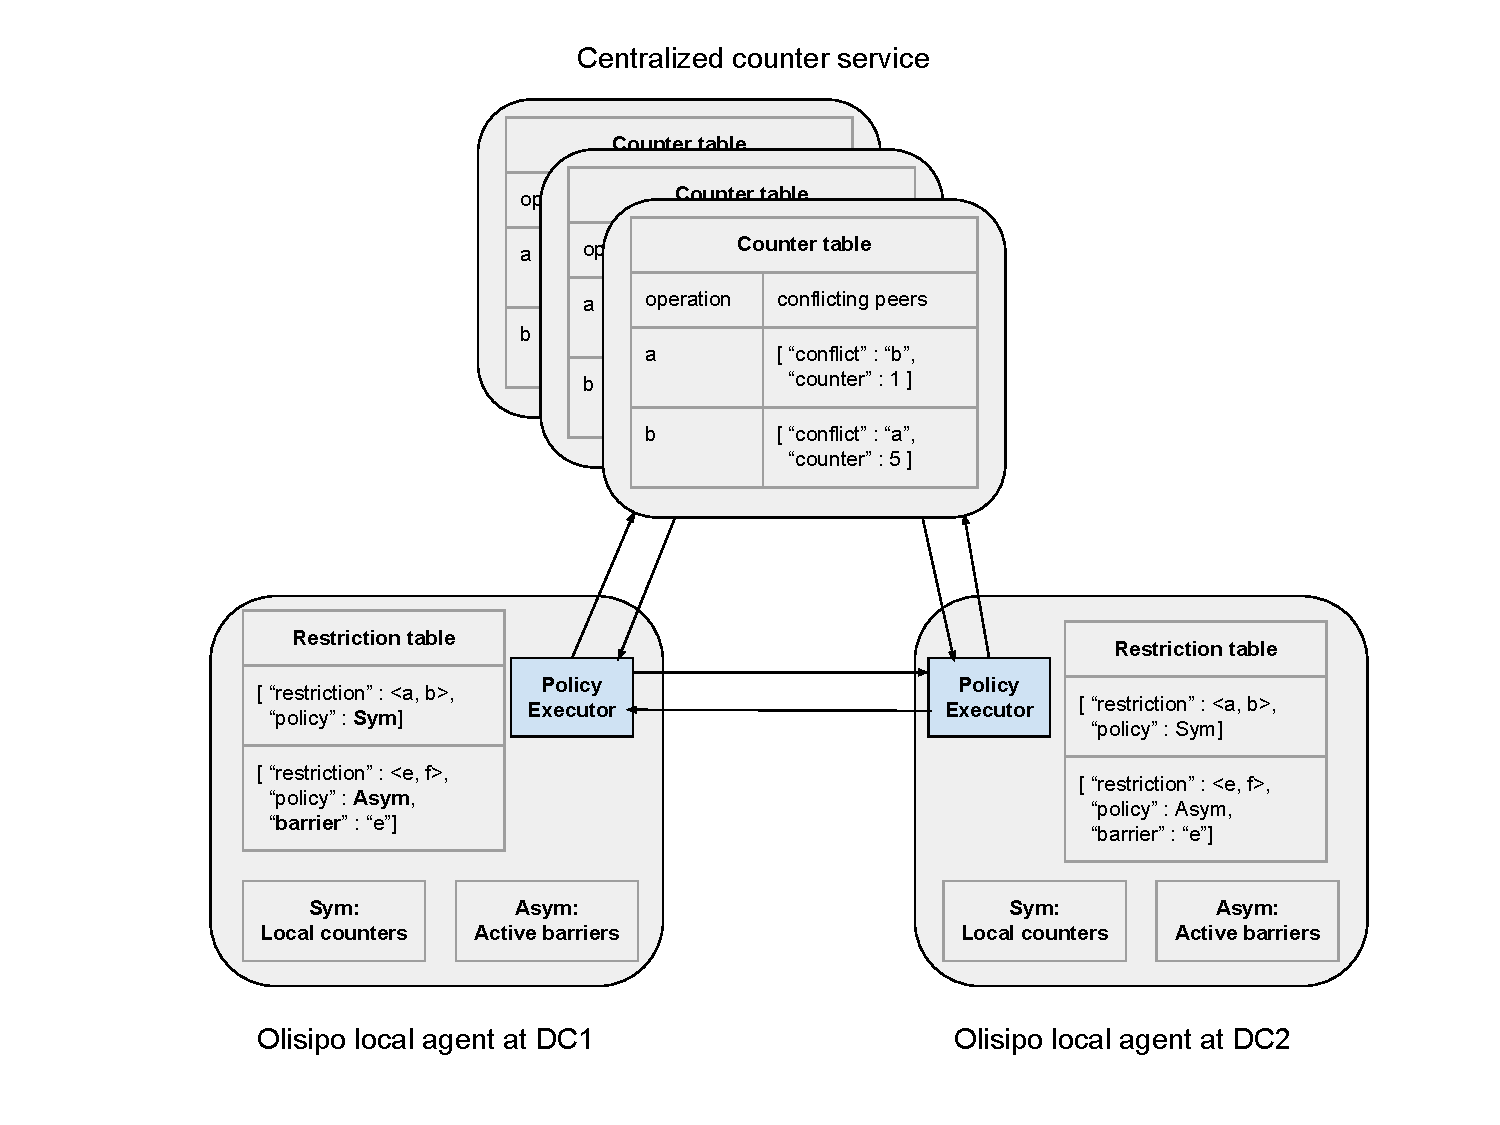
\includegraphics[width=\columnwidth]{./figures/por/tool_support.pdf}
\caption{\coordtool\ architecture}
\label{fig:tooldesign}
\end{figure}

All design choices and details presented above lead to the high level system architecture 
depicted in Figure~\ref{fig:tooldesign}. The \coordtool\ architecture consists of a replicated counter service across data centers and a local agent deployed
in every data center. While the counter service is required by executing the {\tt Sym} protocol
for keeping track of the number of different operations that have been accepted by the system.
the local agent is responsible for placing coordination only when the corresponding
operation is confined by restrictions. Every local agent keeps a restriction table, which defines
all identified restrictions between pair of operations and the corresponding coordination policy.
In addition, every agent also stores some meta data required for different protocols. With regard
to the {\tt Sym} protocol, it maintains a local copy of the replicated counter service, which is used
for learning if the local counters lag behind the global counters, which means
the corresponding data centers have to wait until all missing operations have been locally
incorporated. For the {\tt Asym} protocol, every agent maintains a list of active barriers, which
are used for locally deciding if the counterpart operations of such barriers can proceed or must wait.

\begin{figure}[t!]
\centering
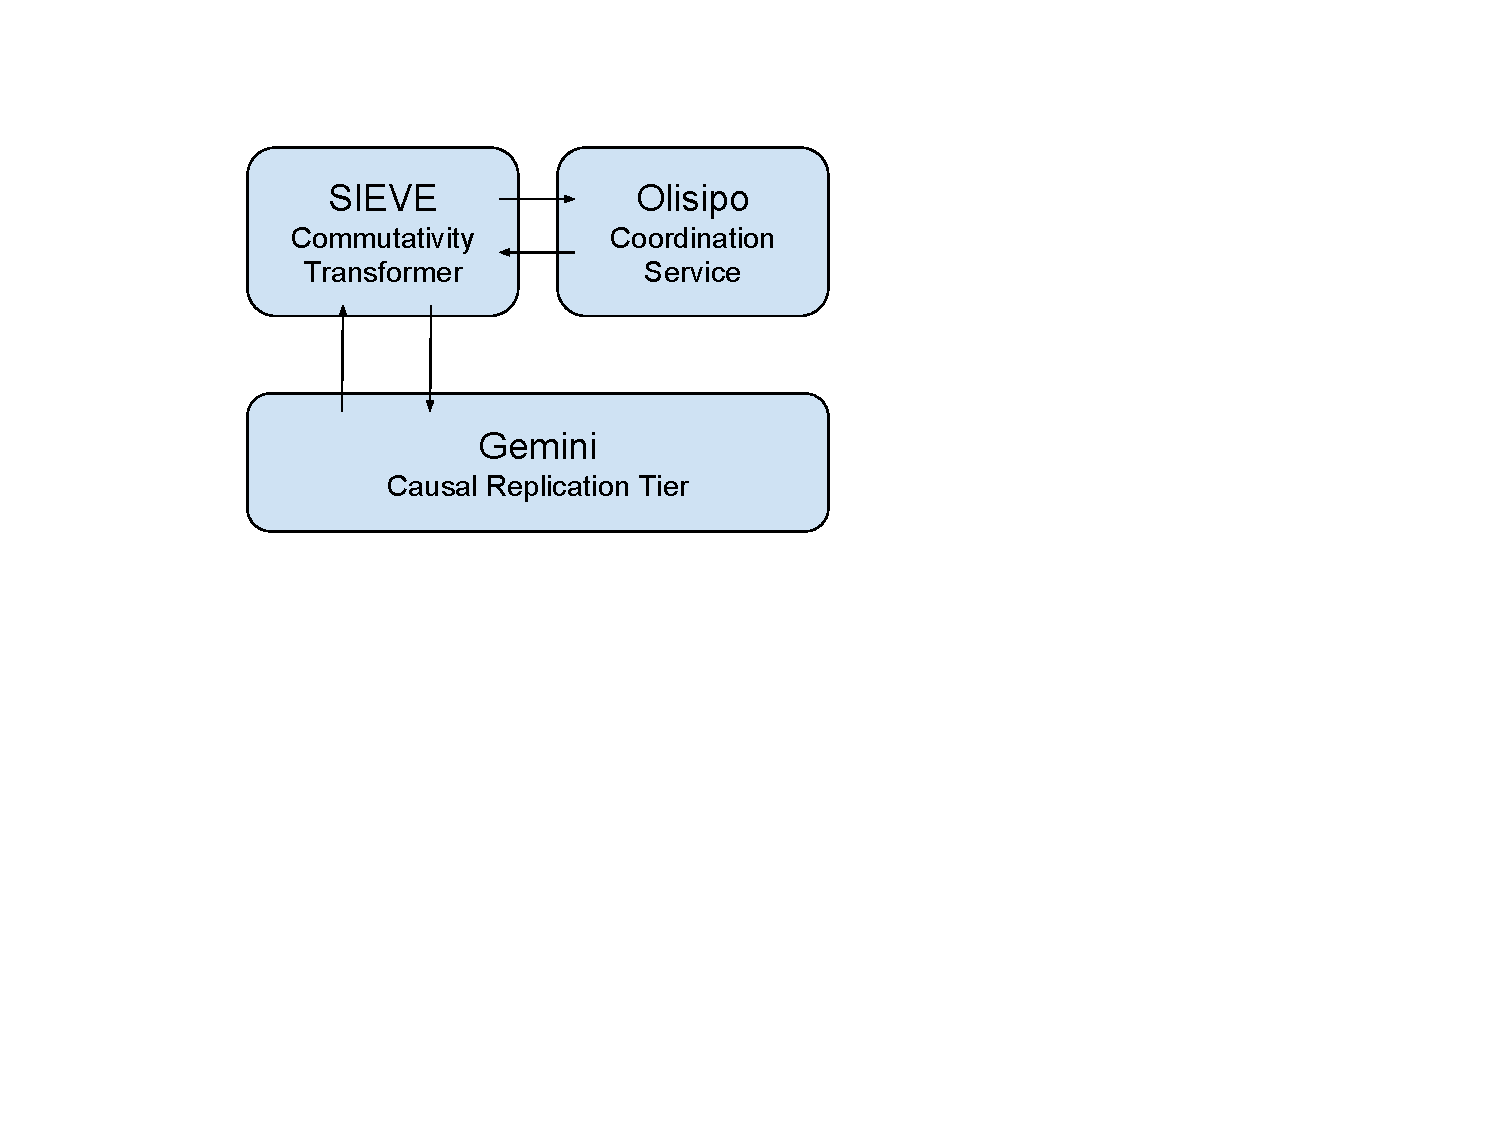
\includegraphics[width=0.76\columnwidth]{./figures/por/tool_intergated.pdf}
\caption{\coordtool\ connected with \tool\ and \gemini}
\label{fig:toolwithenvironment}
\end{figure}

\subsection{Implementation}
We implemented \coordtool\ using Java ($2.8k$ lines of code)~\footnote{The lines of code is
measured by {\tt cloc}~\cite{codecounter}.}, and used BFTSmart~\cite{bftsmartcode} for replicating
the state of the centralized counter service, MySQL as the backend storage, and Netty
as the communication library~\cite{Netty}. As shown in Figure~\ref{fig:toolwithenvironment},
we integrated \coordtool\ with \gemini\ and \tool\ so
that \gemini\ serves as the underlying causally consistent replication tier while \tool\ is used to
produce commutative shadow operations at runtime. 

\noindent\paragraph{Workflow:} A user issues her request to an application server locating at a nearby
data center, which runs a \tool\ library introduced in Chapter~\ref{chapter:sieve} and
a local agent shown in Figure~\ref{fig:tooldesign}. \tool\ intercepts the communication between
the app server and the backend MySQL database and executes the corresponding generator operation.
When the execution ends, \tool\ produces a commutative shadow operation that accumulates side effects
of that request, and then asks the \coordtool\ local agent for placing coordination if needed before committing and replicating
that shadow operation. To do so, \coordtool\ agent lookups into the restriction table
if that operation is confined by any restriction. If so, then the {\tt policy executor} residing
\coordtool\ orders that operation with respect to all its conflicting operations that are running concurrently
at other data centers. This is achieved by invoking a sequence of functions 
presented in Figure~\ref{fig:por:olisipinterface} associated with different protocols 
according to the lookup result, i.e., which protocols to be used. 
At the end, when conflicting operations are accordingly serialized, \tool\ sends these
operations to \gemini\ for replicating them across all data centers while respecting the established order. 
The sourcecode of \coordtool\ is available at ~\cite{olisipocode}.

\begin{landscape}
\begin{table*}[t!]
\centering
\footnotesize
\begin{tabular}{c|c|c|c|c|c|c||c}
\hline
\specialcell{Consistency \\level} & Example systems & \specialcell{Immediate \\response} & \specialcell{State \\convergence} &  \specialcell{Single \\value} & \specialcell{General \\operations}  & \specialcell{Stable\\histories}& \specialcell{Classification \\strategy}\\
\hline
Strong & RSM~\cite{Lamport1978Time,Schneider1990RSM}                & no  & yes  & yes & yes & yes        & N/A\\
\hline
\specialcell{Timeline/\\snapshot} & \specialcell{PNUTS~\cite{Cooper2008PNUTS}, \\Megastore~\cite{Baker2011Megastore}}            & reads only  & yes & yes & yes & yes & N/A\\
\hline
Fork & SUNDR~\cite{Krohn2004Sundr}                                               & all ops & no  & yes  & yes & yes        & N/A\\
\hline
\multirow{3}{*}{Eventual}
& Bayou~\cite{Terry1995Managing}, Depot~\cite{Mahajan2010Depot} & all ops    & yes & no  & yes & yes         & N/A \\
                                   &  Sporc~\cite{Feldman2010Sporc}, CRDT~\cite{Shapiro2011Conflict}                 & all ops       & yes & yes & no & yes          & N/A \\
                                   & Zeno~\cite{Singh2009Zeno}, COPS~\cite{Lloyd2011Causal}  & weak/all ops      & yes & yes  & yes & no         & no / N/A\\
\hline
\multirow{2}{*}{\specialcell{Multi}}   
                                  
                                   & PSI~\cite{Sovran2011PSI}                        & cset         & yes & yes & partial & yes & no\\
                                   &lazy repl.~\cite{Ladin1992LazyReplication}, Horus~\cite{VanRenesse1996Horus}          & immediate/causal ops & yes & yes & yes & yes         & no\\
\hline
\RB\     & \gemini       & \Red\ ops & yes & yes & yes & yes & yes \\
\hline
\end{tabular}
\caption{Tradeoffs in geo-replicated systems and various consistency
  levels.}
\label{table:systemcompare}
\end{table*}
\end{landscape}

\section{Related work}%\pagelimit{1.5}}                                                    
\label{ch:redblue:sect:related}
\if 0
\paragraph{Target end-to-end properties.}
To frame the discussion of existing systems that may be used
for geo-rep\-li\-cat\-ion, we start by informally stating some
desirable properties that such solutions should support.\ The first property consists of ensuring a good user experience by
providing \textbf{low latency} access to the
service~\cite{Schurman2009latency}. Providing low latency access implies
that \operations\ should proceed after contacting a small number of
replicas, but this is at odds with other requirements that are often sacrificed by consistency
models that privilege low latency. The first such requirement is preserving
\textbf{caus\-al\-ity}, both in terms of the monotonicity of user requests
within a session and preserving causality across clients, which is key
to enabling natural semantics~\cite{Petersen1997Flexible}.  Second, it
is important for all \operations\
executed at one replica to be
propagated to all remaining replicas, a property we call
\textbf{eventual propagation}.\ Third, it is important that all
replicas that have executed the same set of \operations\ are in the
same state, i.e., that they exhibit \textbf{state convergence}; otherwise a quiescent system would return different views of the state
depending on which replicas the users connected to. Fourth, we also
want to avoid marked deviations from the conventional, single server
semantics. In particular, \operations\ should return a \textbf{single
  value}, precluding solutions that return a set of values
corresponding to the outcome of multiple concurrent updates; the
system should provide a set of \textbf{stable histories}, meaning that
user actions cannot be undone; and it should provide support for
\textbf{general \operations}, not restricting the type of
\transactions\ that can be executed.  Finally, the behavior of the
service must obey a service-dependent specification, which may be
defined as a set of \textbf{invariants} that must be preserved.
\fi

In this section, we compare several proposals of consistency definitions against our work
by analyzing which set of end-to-end properties described in Chapter~\ref{chapter:sysmodel} they offer.
Table~\ref{table:systemcompare} shows that different proposals strike different balances between
these target properties. While other consistency
definitions exist, we focus on the ones most closely related to the
problem of offering fast and consistent responses in geo-replicated
systems.

\paragraph{ Strong vs.\ weak consistency.}
On the strong consistency side of the spectrum there are definitions
like linearizability~\cite{Herlihy1990Linearizability}, where the
rep\-li\-cated system behaves like a single server that
serializes all \operations.\ This, however, requires coordination among rep\-li\-cas
to agree on the order in which \operations\ are executed, with the
corresponding overheads that are amplified in
geo-rep\-li\-ca\-tion scenarios. Somewhat more efficient are
timeline consistency in PNUTS~\cite{Cooper2008PNUTS} and
snapshot consistency in Megastore~\cite{Baker2011Megastore}. These
systems ensure that there is a
total order for updates to the service state, but give the option
of reading a
consistent but dated view of the service. %new
Similarly, Facebook has a primary site that handles updates
and a secondary site that acts as a read-only copy~\cite{Li2012Practical}.
This allows for fast reads executed at the closest site but writes still pay a penalty for serialization.  
%% These solutions provide fast reads but can result in degraded update
%% performance in situations, like social networking or online shopping
%% services, where a partitioning of the writers of each data item or
%% each group of data items is not easily achievable.
%% %% megastore and pnuts totally order writes but allow for stale reads
%%  The
%% Megastore~\cite{Baker11Megastore} system used by Google uses a
%% modified version of Paxos, requiring all replicas to be contacted
%% during write operations, but enables fast reads at a single replica;
%% % (and thus requires contacting a quorum
%% %of replicas) to serialize write \operations, but
%% %enables reads to read a consistent but dated view from a single replica.
%% \changebars{like PNUTS, this does not allow for fast writes.}{this has same benefits and drawbacks as PNUTS.}
%\rodrigo{Removable:} This system has the additional characteristic of grouping related
%data items in entity groups, and providing full ACID
%semantics within entity groups but lower consistency guarantees across
%the entity boundary. 
Fork consistency~\cite{Krohn2004Sundr, Mazieres2002Fork} addresses
the performance limitations of strong consistency by allowing users to
observe distinct causal histories.  The primary drawback of fork
consistency is that once replicas have forked, they can never be
reconciled.  Such approach is useful when building secure systems
but is not appropriate in the context of geo-replicating a single
service.

Eventual consistency~\cite{Terry1995Managing} is on the other end of the
spectrum. Eventual consistency is a catch-all phrase that covers any
system where replicas may diverge in the short term as long as the
divergence is eventually repaired and may or may not include
causality.  (See Saito and Shapiro~\cite{Saito2005Optimistic} for a
survey.)  In practice, as shown in Table~\ref{table:systemcompare},
systems that embrace weak consistency (e.g., eventual or causal consistency) have limitations. Some
systems waive the stable history property, either by rolling back
\operations\ and re-executing them in a different order at some of the
replicas~\cite{Singh2009Zeno}, or by resorting to a last writer wins
strategy, which often results in loss of one of the
  concurrent updates~\cite{Lloyd2011Causal}.  Other systems expose multiple values from
divergent branches in \operations\ replies either directly to the
client~\cite{Mahajan2010Depot,Decandia2007Dynamo} or to an
application-specific conflict resolution
procedure~\cite{Terry1995Managing}.  Finally, some systems restrict
\operations\ by assuming that all \operations\ in the system
commute~\cite{Feldman2010Sporc,Shapiro2011Conflict}, which might require
the programmer to rewrite or avoid using some \operations.

\paragraph{Coexistence of multiple consistency levels.} The solution we propose for addressing the tension between low latency
and strongly consistent responses is to allow different
\operations\ to run with different consistency
levels. Existing systems that used a similar approach include
Horus~\cite{VanRenesse1996Horus}, lazy replication~\cite{Ladin1992LazyReplication}, Zeno~\cite{Singh2009Zeno}, and
PSI~\cite{Sovran2011PSI}. However, none of these proposals guide the
service developer in choosing between the available consistency
levels.  In particular, developers must reason about wheth\-er their
choice leads to the desired service behavior, namely by ensuring that
invariants are preserved and that replica state does not diverge.
This can be challenging due to difficulties in identifying behaviors
allowed by a specific consistency level and understanding the
interplay between \operations\ running at different levels.  Our
research addresses this challenge, namely by defining a set of
conditions that precisely determine the appropriate
  consistency level for each operation.

\paragraph{Other related work.} Consistency rationing~\cite{Kraska2009ConsisRation} allows consistency
guarantees to be associated with data instead of \operations, and the
consistency level to be automatically switched at runtime between
weak consistency and serializability
based on specified policies.\ TACT~\cite{Yu2000TACT} consistency
bounds the amount of inconsistency of data items in an
application-specific manner, using the following metrics: numerical
error, order error and staleness. In contrast to these models, the
focus of our work is not on adapting the consistency levels of
particular data items at runtime, but instead on systematically
partitioning the space of \transactions\ according to their actions
and the desired system semantics.

One of the central aspects of our work is the notion of
\shadow\ \transactions, which increase \operation\ commutativity by
decoupling the decision of the side effects from their application to the state.
%This enables applications to make more use of fast \transactions. 
Some prior work also aims at increasing operation commutativity: Weihl exploited
com\-mut\-at\-iv\-ity-based concurrency control for abstract data types~\cite{Weihl1988Commutativity}; 
operational transformation~\cite{Ellis1989Concurrency,Feldman2010Sporc} extends
non-co\-mmutative \operations\ with a
transformation that makes them commute; Conflict-free Replicated Data
Types (CRDTs)~\cite{Shapiro2011Conflict} design \operations\ that
commute by construction; Gray~\cite{Gray1981NestedTransactions} proposed
an open nested transaction model that uses commutative compensating
transactions to revert the effects of aborted transactions without
rolling back the transactions that have seen their results and already
committed; delta transactions~\cite{deltaTxBlog} divide a transaction
into smaller pieces that commute with each other to reduce the
serializability requirements.  Our proposal of
\shadow\ \transactions\ can be seen as an extension to these concepts,
providing a different way of broadening the scope of potentially commutative
\transactions. There exist other proposals that also decouple the
execution into two parts, namely two-tier
replication~\cite{Gray1996Dangers} and CRDT
downstreams~\cite{Shapiro2011Conflict}. In contrast to these proposals, for
  each \operation, we may generate different
  \shadow\ \operations\ based on the specifics of the execution,
which can run under different consistency levels. As a result, the decomposition enables a
dynamic runtime classification of consistency levels, and
allows applications to make more use of fast \operations.


\section{Conclusion}
This paper proposed a research direction for building replicated system that employs a minimal amount of coordination in
order to achieve both invariant preservation and state convergence. We aim to define a new generic consistency model, which \changebars{maps
consistency requirements to a minimal set of fine-grained restrictions over pairs of operations}{allows to
capture a set of minimum coordination restrictions to ensure the desired properties}, while at the same time paving the way for adaptive use of different coordination
techniques for enforcing those restrictions.

{\footnotesize
\acks

The research of R.\ Rodrigues is funded by the European
Research Council under ERC Starting Grant No.\ 307732. This work is
partially funded by FCT under project PEst-OE/EEI/UI0527/2014.
}
% We recommend abbrvnat bibliography style.

\bibliographystyle{abbrvnat}
{%\footnotesize
\scriptsize
\bibliography{sigproc}
}

\end{document}

%                       Revision History
%                       -------- -------
%  Date         Person  Ver.    Change
%  ----         ------  ----    ------

%  2013.06.29   TU      0.1--4  comments on permission/copyright notices

